\documentclass[conference]{IEEEtran}
% Times için T1: tectonic (XeTeX) TU kodlamasında ptm bulamıyor; pdflatex'te zararsız.
\usepackage[T1]{fontenc}
\usepackage{cite}
\usepackage{amsmath}
\usepackage{graphicx}
\usepackage{booktabs}
\usepackage{url}
\usepackage[hidelinks]{hyperref}

\begin{document}

\title{Floor Plan Parsing Without Learned Models:\\
Walls, Openings and Room Graphs}

% Ekip üyeleri henüz kayıtlı değil; eklenecek.
\author{\IEEEauthorblockN{\"Omer Can Atl\i{}}
\IEEEauthorblockA{Department of Computer Engineering\\
Gebze Technical University\\
Kocaeli, T\"urkiye}}

\maketitle

\begin{abstract}
We present a rule-based parser that converts a raster architectural floor
plan into walls, doors, windows, rooms and a room--door graph using only
classical image processing: thresholding, mathematical morphology, the
progressive probabilistic Hough transform, template matching and the
watershed transform. No learned model is used at any stage. Walls are
extracted at two morphological scales and vectorized from their skeleton;
openings are found as gaps between wall ends and classified by fitting
quarter-circle door arcs and parallel window lines; rooms are segmented by
closing the openings and splitting the free space with a distance-transform
watershed. On the solid-wall subset of the CVC-FP dataset, measured once on a
held-out test split of 24 plans, the method reaches a wall pixel IoU of
0.913, door F1 0.904, window F1 0.830 and room F1 0.770 under strict
one-to-one matching at IoU $\geq 0.5$. All thresholds were chosen on a
separate development split of 62 plans. We compare against published
results on the same data, analyze the remaining errors, and report the
drawing styles where the approach fails.
\end{abstract}

\begin{IEEEkeywords}
floor plan analysis, document image analysis, mathematical morphology,
Hough transform, template matching, watershed segmentation
\end{IEEEkeywords}

\section{Introduction}

Architectural floor plans are routinely exchanged as raster images in which
the semantic structure (which strokes are walls, where the doors are, which
spaces are rooms) is lost. Recovering that structure is a classical problem
of graphics recognition~\cite{mace2010rooms,ahmed2011improved,delasheras2014statistical}.
Recent work relies mostly on trained detectors and segmentation
networks~\cite{dodge2017parsing,liu2017raster,kalervo2019cubicasa,santhosh2026flooryolo}.
This project deliberately does not: the task, set for an image processing
course, is to solve the problem with classical operators only, so that every
decision of the system can be traced to a measurable image property.

The contributions of this work are:
\begin{itemize}
\item a complete pipeline from pixels to a room--door graph built only from
thresholding, morphology, Hough lines, template matching and the watershed
transform;
\item geometric tests for openings: gap candidates from wall ends and mask
corners, a four-hypothesis quarter-arc template for doors, and line- and
arc-based tests for single and double casement windows;
\item an evaluation protocol with strict one-to-one matching for every
element type, a development/test split fixed in advance, and a single test
measurement, together with an error analysis that separates fixable
failures from failures the approach cannot address.
\end{itemize}

\section{Related Work}

Mac\'e et al.~\cite{mace2010rooms} detect rooms by separating thick and thin
lines, finding walls and doors with Hough-based primitives, and decomposing
the remaining space. Ahmed et al.~\cite{ahmed2011improved} extend this with a
three-way thick/medium/thin separation and a building boundary, and later add
text labels from OCR to split rooms that have no physical
separation~\cite{ahmed2012rooms}. Their evaluation uses the protocol of
Phillips and Chhabra~\cite{phillips1999evaluation}, which gives partial
credit for one-to-many and many-to-one matches.

De las Heras et al.\ introduced patch-based wall
segmentation~\cite{delasheras2011patch}, a full statistical and structural
pipeline~\cite{delasheras2014statistical}, and the CVC-FP
dataset~\cite{delasheras2015cvcfp} used here. Dodge et
al.~\cite{dodge2017parsing} compare thresholding, patch classifiers and fully
convolutional networks for wall segmentation on CVC-FP. Swaileh et
al.~\cite{swaileh2021versailles} generate wall masks for historical plans
with connected-component filtering and steerable filters before training a
U-Net. Cabrera Vargas~\cite{cabrera2018walls} studies walls and rooms in
multi-unit plans, and Rezvanifar~\cite{rezvanifar2021symbols} spots symbols,
including door arcs found by partial-ellipse voting. FloorYOLO~\cite{santhosh2026flooryolo}
detects doors and windows on CVC-FP with an attention-augmented YOLOv8n.

We did not find a published system that extracts walls, doors, windows,
rooms and the room--door graph on CVC-FP without any learned component and
reports all of them; the closest is~\cite{delasheras2014statistical}, whose
full text we could not access.

\section{Data and Evaluation}

\subsection{Dataset and split}

CVC-FP~\cite{delasheras2015cvcfp} contains 122 annotated plans in four
drawing styles. Walls, rooms, doors, windows, wall-less separations and
parking (garage) objects are annotated as polygons, and rooms are linked to their doors
by \emph{access} relations. The largest group (90 plans,
$2479\times3508$\,px) draws walls as solid black bands in 86 plans; the
other styles use hatched fills or double outlines. The method targets solid
walls; we report the solid-wall subset as the main result and all styles
separately.

There is no official split. We hold out 30\% of each style group by the
SHA-1 order of the plan names: 86 development and 36 test plans (62 and 24
solid-wall plans). Every threshold and design choice was made on the
development plans; the test plans were evaluated once, after the method was
frozen.

\subsection{Metrics}

\emph{Walls:} pixel IoU between the predicted wall mask and the union of the
ground-truth wall polygons, averaged over plans. \emph{Doors and windows:}
each predicted polygon is matched to at most one ground-truth polygon,
greedily by decreasing IoU, and counts as correct if the IoU is at least
0.5; we also report the same matching on axis-aligned bounding boxes for
comparison with object detectors. \emph{Rooms:} the same one-to-one rule
between predicted room regions and ground-truth room polygons.
\emph{Graph edges:} a predicted room--door--room edge is correct if its door
matches a ground-truth door, both rooms match ground-truth rooms, and the
ground truth links that door to exactly those two rooms. Precision (P),
recall (R) and F1 are computed from the pooled counts.

These metrics are strict. Merging two rooms counts as one miss and one
false region, with no partial credit, unlike the DR/RA protocol used
in~\cite{ahmed2011improved,ahmed2012rooms}.

\section{Method}

Fig.~\ref{fig:pipeline} shows the stages on a crop of a development plan.

\begin{figure*}[t]
\centering
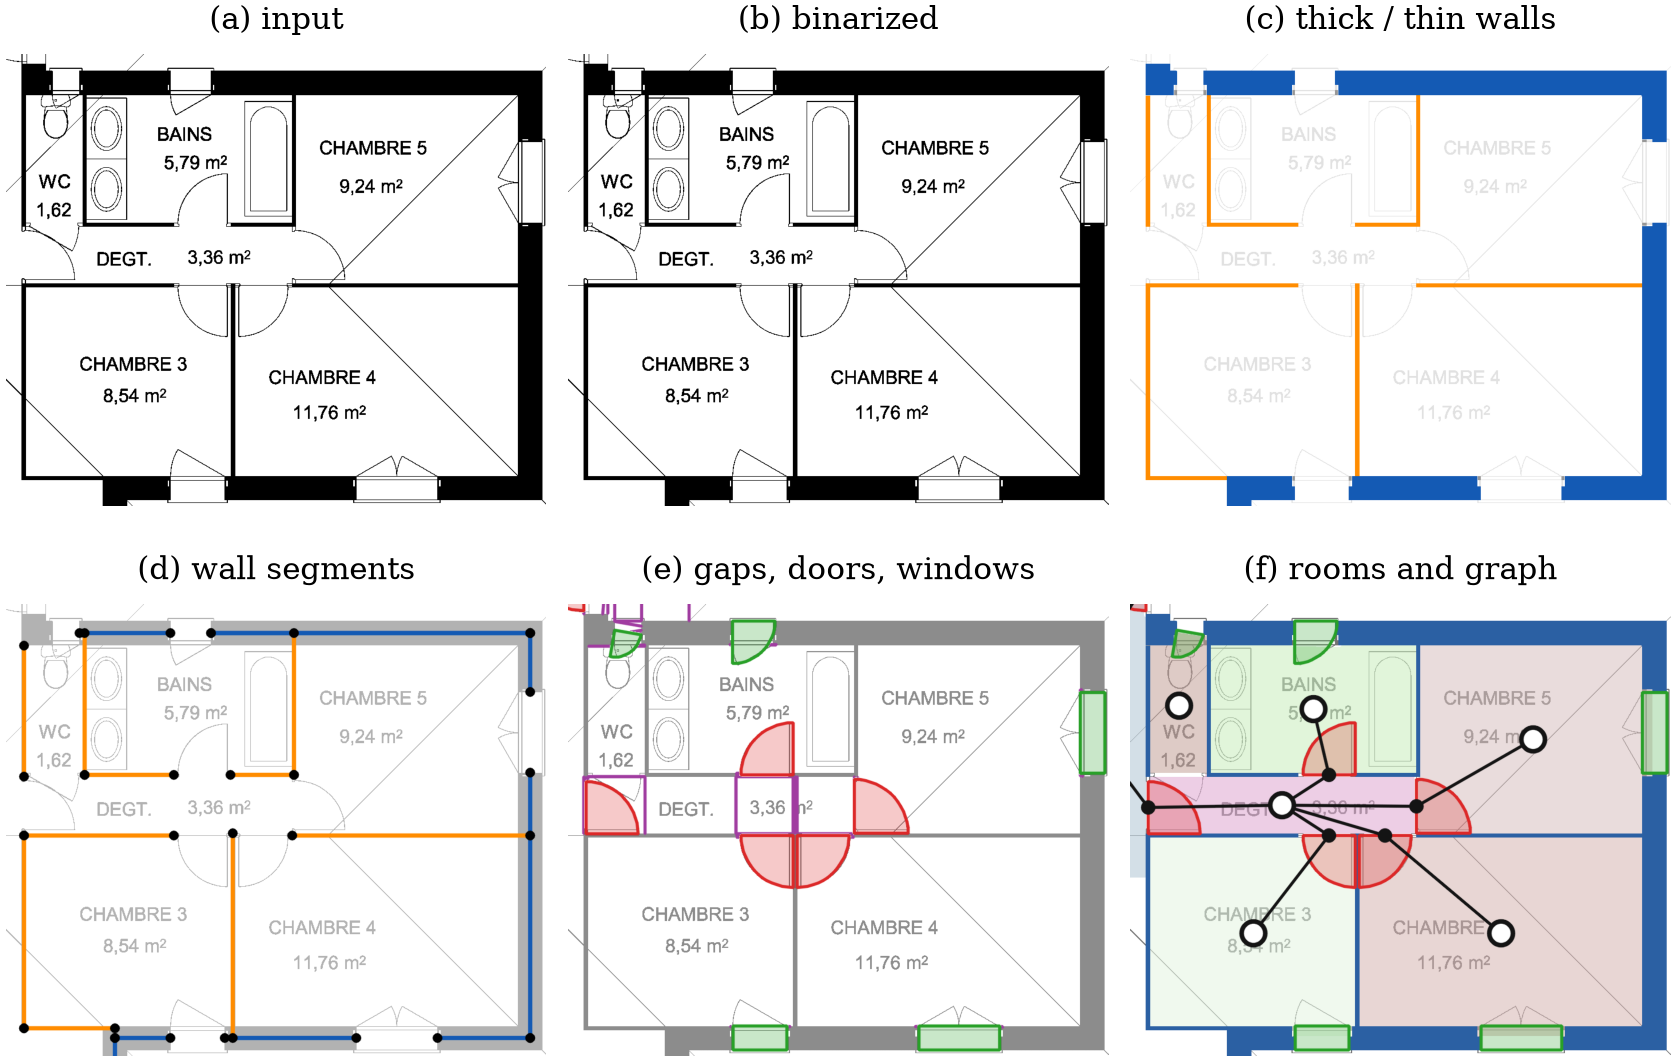
\includegraphics[width=\textwidth]{sekiller/pipeline.png}
\caption{Pipeline stages on a development plan. (c)~Thick mask (blue),
thin-scale candidates (gray) and thin walls accepted by the rules
(orange). (d)~Wall segments from the skeleton and Hough transform, with
their end points. (e)~Gap candidates (purple), detected doors (red) and
windows (green). (f)~Rooms and the room--door graph.}
\label{fig:pipeline}
\end{figure*}

\subsection{Preprocessing}

The grayscale image is binarized with Otsu's threshold~\cite{otsu1979threshold}.
Enclosed paper regions of at most 4 pixels, which occur inside scanned wall
bands, are filled.

\subsection{Two-scale wall mask}

A single morphological opening~\cite{soille2003morphological} cannot
separate thin partition walls (about 7--9\,px) from strokes of the same
width such as stair treads. We therefore use two scales. The \emph{thick}
mask is the opening with a $13\times13$ square and is accepted as wall
directly. The \emph{thin} candidates are the opening with a $7\times7$
square minus the dilated thick mask; they are vectorized (Section~IV-C) and
a thin segment is accepted as a wall only if it is at least 30\,px long, its
median transverse width is at most 10\,px, its width varies little
(interquartile range at most 0.2 of the median), and it has at most one
parallel neighbor within 60\,px (stair treads come in parallel series).

A square structuring element is direction dependent: a $7\times7$ square
fits into a $45^\circ$ band only if the band is about $7\sqrt{2}$\,px wide,
so thin diagonal walls disappear. The pixels kept by an opening with a
7\,px disk but not by the square opening form a separate mask; segments
from that mask that are at least $10^\circ$ off both axes and pass the same
thin-wall rules are added. Keeping the square candidates unchanged and only
adding diagonal segments matters: merging the disk opening into the
candidate mask shifted existing segments and changed downstream results.

\subsection{Vectorization}

Each mask is thinned~\cite{zhang1984thinning} and line segments are found
with the progressive probabilistic Hough transform~\cite{matas2000pphough}
(accumulator threshold 10, minimum length 15\,px, maximum gap 20\,px).
Collinear segments (angle within $3^\circ$, offset within 3\,px, gap within
20\,px) are merged; each segment is extended along its direction to the mask
boundary, its thickness is measured as the median transverse extent at
quarter-pixel steps, and end points near another wall (angle at least
$20^\circ$) are moved to the intersection of the two center lines. The final
wall mask is the thick mask plus the rectangles of the accepted thin
segments.

\subsection{Gap candidates}

Openings appear as interruptions of wall lines. From each segment end a ray
is cast along the segment; if it leaves the wall and meets wall again after
40--200\,px, the free interval is a candidate gap. At an end that is joined
to another wall the ray first crosses that wall, and the wall it meets must
be collinear (within $10^\circ$); otherwise the ray would cross the room
from a T-junction. Further candidates come from rays along both faces of
every approximately right-angled convex corner of the wall mask, which
covers short or slanted wall ends that produced no segment. Gaps of
150--450\,px are searched separately for wide windows; there the opposite
wall must be collinear, or be a short pier whose local transverse width
matches the source wall.

\subsection{Doors}

A door is drawn as a leaf and a quarter-circle arc centered at the hinge.
For a gap of width $g$ we test four hypotheses (hinge at either end, opening
to either side), with the hinge on the wall face or on its center line, and
radii $r \in \{0.85, 0.92, 1.0, 1.06\}\,g$; for door-size arcs
($r \geq 75$\,px) the radii $0.83g$ to $1.07g$ in steps of $0.04g$ are added.
For each hypothesis 24 points of the
quarter arc between $8^\circ$ and $82^\circ$ are sampled; the score is the
fraction of points within 3\,px of thin ink, i.e.\ the binary image with
the dilated wall mask removed. A gap is a door if the best score is at least
0.8 and $r \geq 75$\,px; smaller arcs are casement windows. Overlapping
detections are suppressed by the IoU of their swing sectors.

The radius step matters. With a step of about 7\,px, twice the point
tolerance, the correct radius can fall between two tested values
(Fig.~\ref{fig:radius}); adding the intermediate radii for door-size arcs
found 32 more doors on the development set with an unchanged window F1.
Applying them to the smaller casement-window arcs as well turned windows
drawn with parallel lines into casement detections and lowered window F1,
so they are limited to door-size arcs.
Candidates from junction ends that hit a perpendicular wall face (doors
at the foot of a T-junction) are tested for arcs only.

\begin{figure}[t]
\centering
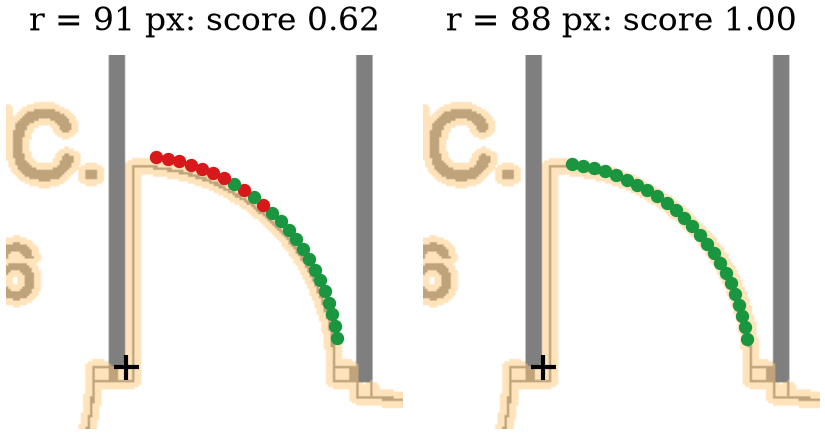
\includegraphics[width=\columnwidth]{sekiller/door_radius.png}
\caption{Arc template on a development plan. Samples within 3\,px of thin
ink are green, others red. A radius of 91\,px, from the original coarse
radius scan, scores 0.62 and the door is missed; the true radius, 88\,px,
scores 1.00.}
\label{fig:radius}
\end{figure}

\subsection{Windows}

In a gap without a door, a window is reported if at least two parallel ink
runs, each covering at least 80\% of the gap, lie inside the wall band. A
double casement window has two leaves hinged at both ends of the gap that
meet in the middle; we test two arcs of radius $g/2$ and require both to
score at least 0.8. Following the ground-truth convention, the polygon of a
casement window is the gap rectangle together with the swing sectors.

\subsection{Rooms and graph}

The closed mask is the wall mask plus 5\,px beams across detected doors,
windows and wide openings, across half-open doors (a partial arc plus a leaf
at $30^\circ$, $45^\circ$ or $60^\circ$, score at least 0.95, used for
closing only) and across the remaining gap candidates. A beam is not drawn
from a wall end that lies on an interrupted wall line, i.e.\ with wall on
both sides within 220\,px: such ends are typically partitions meeting a
corridor between two doors, and their rays cut the corridor.

The building footprint is the closing of the wall mask, with wide openings
closed, by a $301\times301$ square, with holes filled. Regions inside the
footprint whose boundary is less than 80\% wall or beam are concave
exterior spaces such as terraces. The free space is split by a
watershed~\cite{vincent1991watershed} on the distance transform, with
markers where the distance to the nearest wall is at least 45\,px (about
half a door width); adjacent basins merge when the saddle between them is
at least 0.8 of the smaller peak, so that L-shaped rooms stay whole while
rooms joined by an unclosed doorway are separated. Regions of at least
5000\,px are rooms. For every door, the labels a few pixels on both sides of
the door line give a room--room or room--exterior edge in a multigraph.

\begin{figure*}[t]
\centering
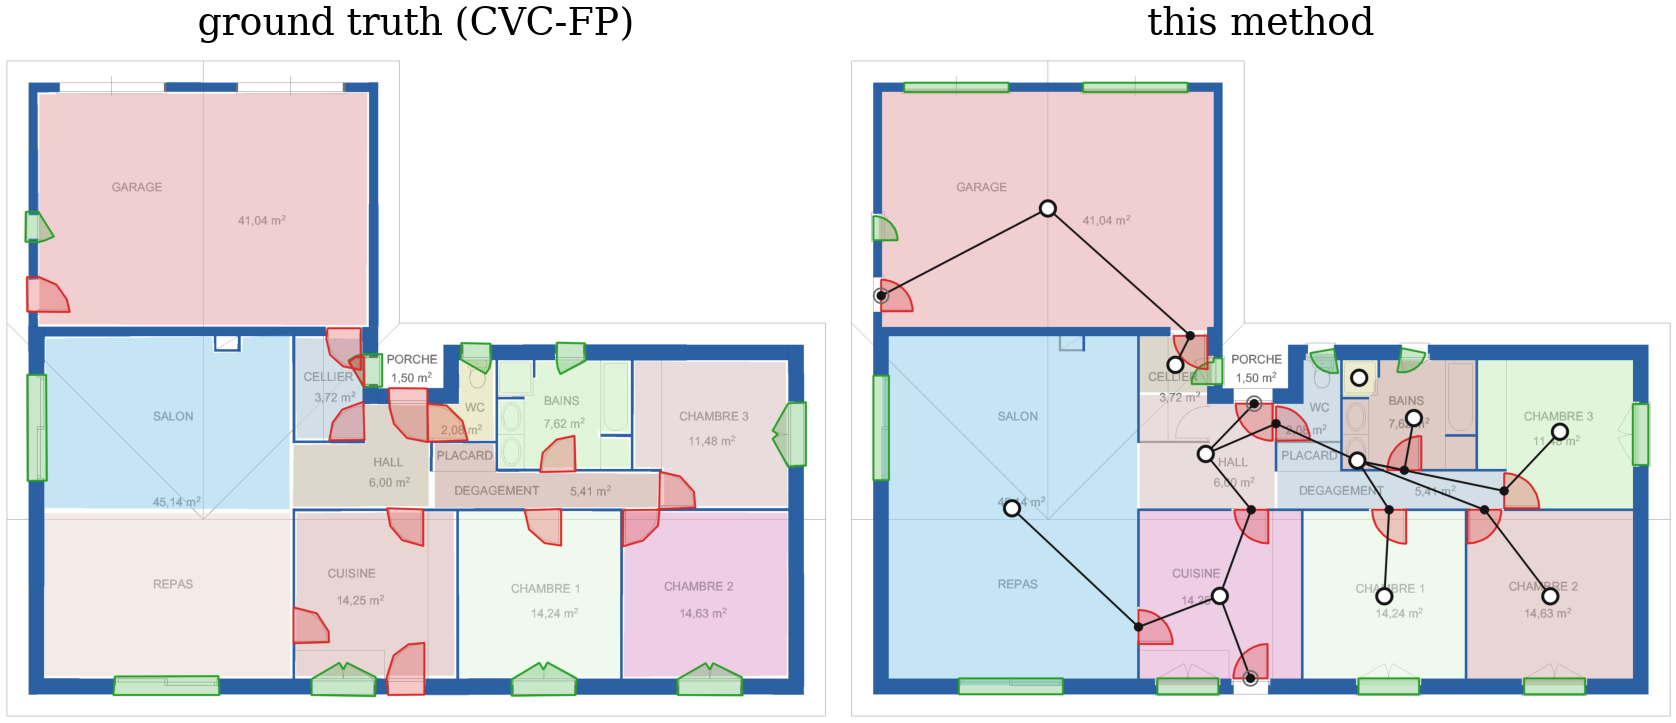
\includegraphics[width=0.92\textwidth]{sekiller/test_example.png}
\caption{Test plan with the median room F1 (0.78). Walls blue, doors red,
windows green, rooms in pastel colors; right: the room--door graph. Salon
and dining area are one room in our output: the ground truth separates them
without a wall.}
\label{fig:example}
\end{figure*}

\section{Results}

\subsection{Test results}

Table~\ref{tab:main} gives the single test measurement next to the
development results on which the method was tuned. On the solid-wall plans,
wall, door, window and room scores differ by at most 0.015 between the two
splits. The edge F1 is notably higher on the test split; it is computed
from only 188 test edges and depends on whether the corridor, to which most
doors connect, is found as one room, so we do not read the difference as an
improvement. Fig.~\ref{fig:example} shows the test plan with the median room
F1.

\begin{table}[t]
\centering
\caption{Development and test results, solid-wall plans
(P / R / F1; one-to-one matching at IoU $\geq 0.5$).}
\label{tab:main}
\begin{tabular}{lcc}
\toprule
 & development (62) & test (24) \\
\midrule
wall pixel IoU & 0.909 & 0.913 \\
doors & 0.957 / 0.836 / 0.892 & 0.985 / 0.835 / 0.904 \\
windows & 0.882 / 0.798 / 0.838 & 0.863 / 0.798 / 0.830 \\
rooms & 0.859 / 0.719 / 0.783 & 0.825 / 0.722 / 0.770 \\
room--door edges & 0.446 / 0.350 / 0.392 & 0.580 / 0.441 / 0.502 \\
\midrule
\multicolumn{3}{l}{all styles (86 / 36 plans), F1} \\
doors & 0.730 & 0.770 \\
windows & 0.652 & 0.625 \\
rooms & 0.647 & 0.651 \\
\bottomrule
\end{tabular}
\end{table}

\subsection{Development history}

Table~\ref{tab:ablation} lists the main design steps and their effect on the
development set. Each step was introduced after classifying the remaining
errors of the previous version; the classification scripts are part of the
repository.

\begin{figure*}[t]
\centering
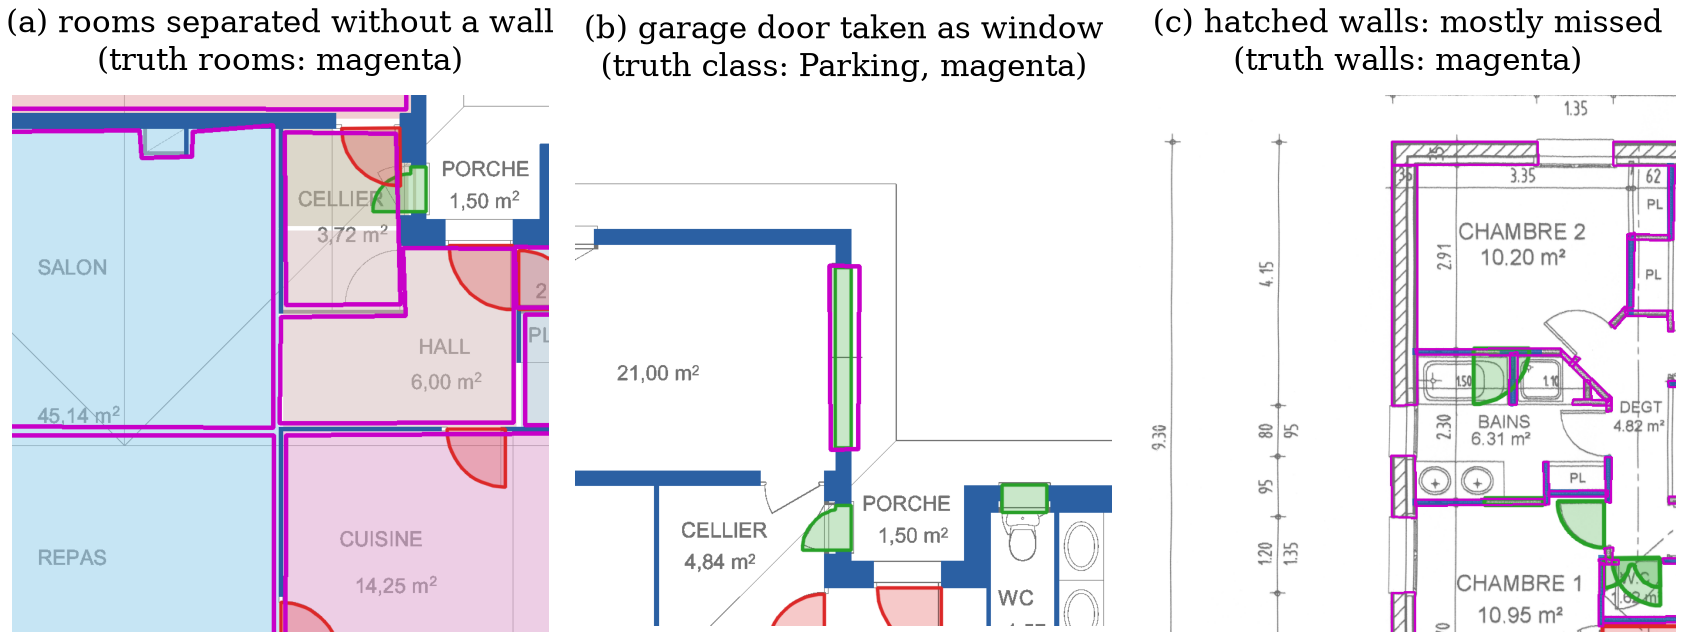
\includegraphics[width=\textwidth]{sekiller/failures.png}
\caption{Failure types. (a)~Two ground-truth rooms separated without a wall
are one region (test plan). (b)~A garage door, annotated as a separate
\emph{parking} object, is detected as a wide window. (c)~Hatched walls
(another drawing style) are mostly missed.}
\label{fig:failures}
\end{figure*}

\begin{table}[t]
\centering
\caption{Effect of design steps on the development set (F1).}
\label{tab:ablation}
\begin{tabular}{lc}
\toprule
step & F1 \\
\midrule
\multicolumn{2}{l}{\emph{walls (median pixel IoU)}} \\
single opening & 0.84 \\
two scales with thin-wall rules & 0.926 \\
\midrule
\multicolumn{2}{l}{\emph{windows}} \\
parallel lines and small arcs & 0.671 \\
+ double casement test & 0.771 \\
+ wide gaps, short piers & 0.839 \\
\midrule
\multicolumn{2}{l}{\emph{doors}} \\
arc score $\geq 0.8$, $r \geq 75$\,px & 0.854 \\
+ finer radius scan, T-junction gaps & 0.885 \\
+ diagonal thin walls & 0.892 \\
\midrule
\multicolumn{2}{l}{\emph{rooms}} \\
connected components & 0.534 \\
+ wide openings, footprint wall share & 0.626 \\
+ watershed splitting & 0.706 \\
+ beam filter, half-open doors & 0.734 \\
+ door and wall improvements & 0.783 \\
\bottomrule
\end{tabular}
\end{table}

\subsection{Comparison with published results}

Table~\ref{tab:literature} collects published numbers on CVC-FP. None of
them uses our protocol and the comparison must be read with the differences
in mind. Dodge et al.\ report the wall Jaccard index on all 122 plans with
five-fold cross-validation; our all-style mean IoU (0.634 on the test split)
lies close to their thresholding baselines and well below the learned
models, because the method finds almost no walls in hatched styles. On
solid walls our 0.913 exceeds the only classical mask generation we found,
0.831 by Swaileh et al., whose input had a textured background added.
FloorYOLO reports precision and recall on a 25-plan validation split of all
styles at $640\times640$ input; our door recall is higher on solid-wall
plans and lower over all styles, and our window detection is below theirs.
The room numbers of Mac\'e et al.\ and Ahmed et al.\ give partial credit to
split and merged rooms and are not directly comparable to our strict
one-to-one recall and precision.

\begin{table}[t]
\centering
\caption{Published results on CVC-FP and ours (test split).}
\label{tab:literature}
\setlength{\tabcolsep}{3pt}
\small
\begin{tabular}{llc}
\toprule
work & setting & value \\
\midrule
\multicolumn{3}{l}{\emph{walls, Jaccard index / IoU}} \\
Dodge~\cite{dodge2017parsing} & Otsu / + morphology & 0.415 / 0.619 \\
 & patches + RF / FCN-2s & 0.792 / 0.892 \\
Swaileh~\cite{swaileh2021versailles} & classical, solid walls & 0.831 \\
ours & all styles, mean / pooled & 0.634 / 0.411 \\
ours & solid walls & 0.913 \\
\midrule
\multicolumn{3}{l}{\emph{doors, box P / R}} \\
FloorYOLO~\cite{santhosh2026flooryolo} & all styles & 0.810 / 0.786 \\
ours & all styles & 0.966 / 0.640 \\
ours & solid walls & 0.985 / 0.835 \\
\midrule
\multicolumn{3}{l}{\emph{windows, box P / R}} \\
FloorYOLO~\cite{santhosh2026flooryolo} & all styles & 0.791 / 0.727 \\
ours & solid walls & 0.671 / 0.621 \\
\midrule
\multicolumn{3}{l}{\emph{rooms (DR / RA, partial credit)}} \\
Mac\'e~\cite{mace2010rooms}$^\ast$ & 80 plans & 0.85 / 0.69 \\
Ahmed~\cite{ahmed2011improved} & same 80 plans & 0.89 / 0.79 \\
Ahmed~\cite{ahmed2012rooms} & + OCR room labels & 0.85 / 0.82 \\
\multicolumn{3}{l}{\emph{rooms (R / P, strict one-to-one)}} \\
ours & solid walls & 0.722 / 0.825 \\
\bottomrule
\multicolumn{3}{l}{\footnotesize $^\ast$as reported in~\cite{ahmed2011improved}.}
\end{tabular}
\end{table}

\subsection{Runtime}

The pipeline runs on a CPU in a median of 6--7\,s per plan of
$2479\times3508$\,px (Python, OpenCV, scikit-image), with arc tests and
watershed segmentation taking most of the time.

\section{Error Analysis and Limitations}

Fig.~\ref{fig:failures} shows the main failure types. In our error analysis
on the development set, 93 of the 602 ground-truth rooms were merged with a
neighbor from which the ground truth separates them without a wall
(Fig.~\ref{fig:failures}a); no geometric
cue exists in the drawing, which caps room recall at about 0.85 for this
approach. Ahmed et al.~\cite{ahmed2012rooms} address this with OCR of room
labels. Most other room merges occur where the door between two rooms was
not found; the remaining missed doors are mostly drawn half open or lie in
walls that the wall step missed. Garage doors, which CVC-FP annotates as a
separate \emph{parking} class, are detected as wide windows
(Fig.~\ref{fig:failures}b). Stair base lines that are as thick as partition
walls and touch no wall are accepted as walls; rules to reject them removed
more true walls than false ones.

The thresholds are in pixels and tied to the scan resolution of CVC-FP; a
different scale would need them rescaled, for example from the median wall
thickness. Hatched and double-outline wall styles are outside the scope
(Fig.~\ref{fig:failures}c): the morphological wall model assumes solid
bands.

\section{Conclusion}

A pipeline built only from classical operators recovers walls, doors,
windows and rooms of solid-wall floor plans with test F1 scores between
0.77 and 0.90 and a wall IoU above 0.91, and its errors can be traced to
specific geometric causes. The largest remaining error, rooms separated
without a wall, cannot be solved from the drawing geometry alone; reading
room labels and normalizing the pixel thresholds by the measured wall
thickness are the natural next steps.

\bibliographystyle{IEEEtran}
\bibliography{refs}

\end{document}
